
%% I'm Finalizing this

\section{Why AC susceptometer?}
It is better to first address the need of The AC susceptometer, in fact susceptometer in general. Susceptomter is an instrument which measures magnetization of sample respect to applied the field. The need of a susceptometer starts with the importance of magnetic properties of material. Magnetic properties are very important in classification of materials and most importantly its behavior in certain conditions. We will see why susceptometry is important by looking at these two cases.

\subsection{Classification of material by its magnetic properties}
Certainly the importance of classification in fields such as material science, chemistry, geology etc is very important. This classification is done by looking at its magnetization properties. For lay people, certain materials such as iron, nickel  are very attractive to magnets but certain materials such as water, mercury are repelled by it. These properties can be deeply understood by looking at its atomic structure and some knowledge of quantum mechanical concepts such as spins of electrons and magnetic moments. By studying magnetic properties which can classify material in certain broad categories.

\subsubsection{Paramagnetic materials}

Most chemical elements and certain compounds show very little magnetization in direction of applied magnetic fields; this material is called paramagnetic materials. This material has very small but positive magnetic susceptibility. Their relative permeability is slightly greater than 1. Paramagnetism is due to unpaired electrons in the materials, so most elements with incomplete orbits have this property. There are theories which try to understand magnetism. 
\begin{itemize}
\item Curie’s law: Paramagnets approximately follow this law which says that magnetization is inversely proportional to its temperature $\chi \propto \frac{1}{T}$.
\begin{figure}[hbt!]\centering
  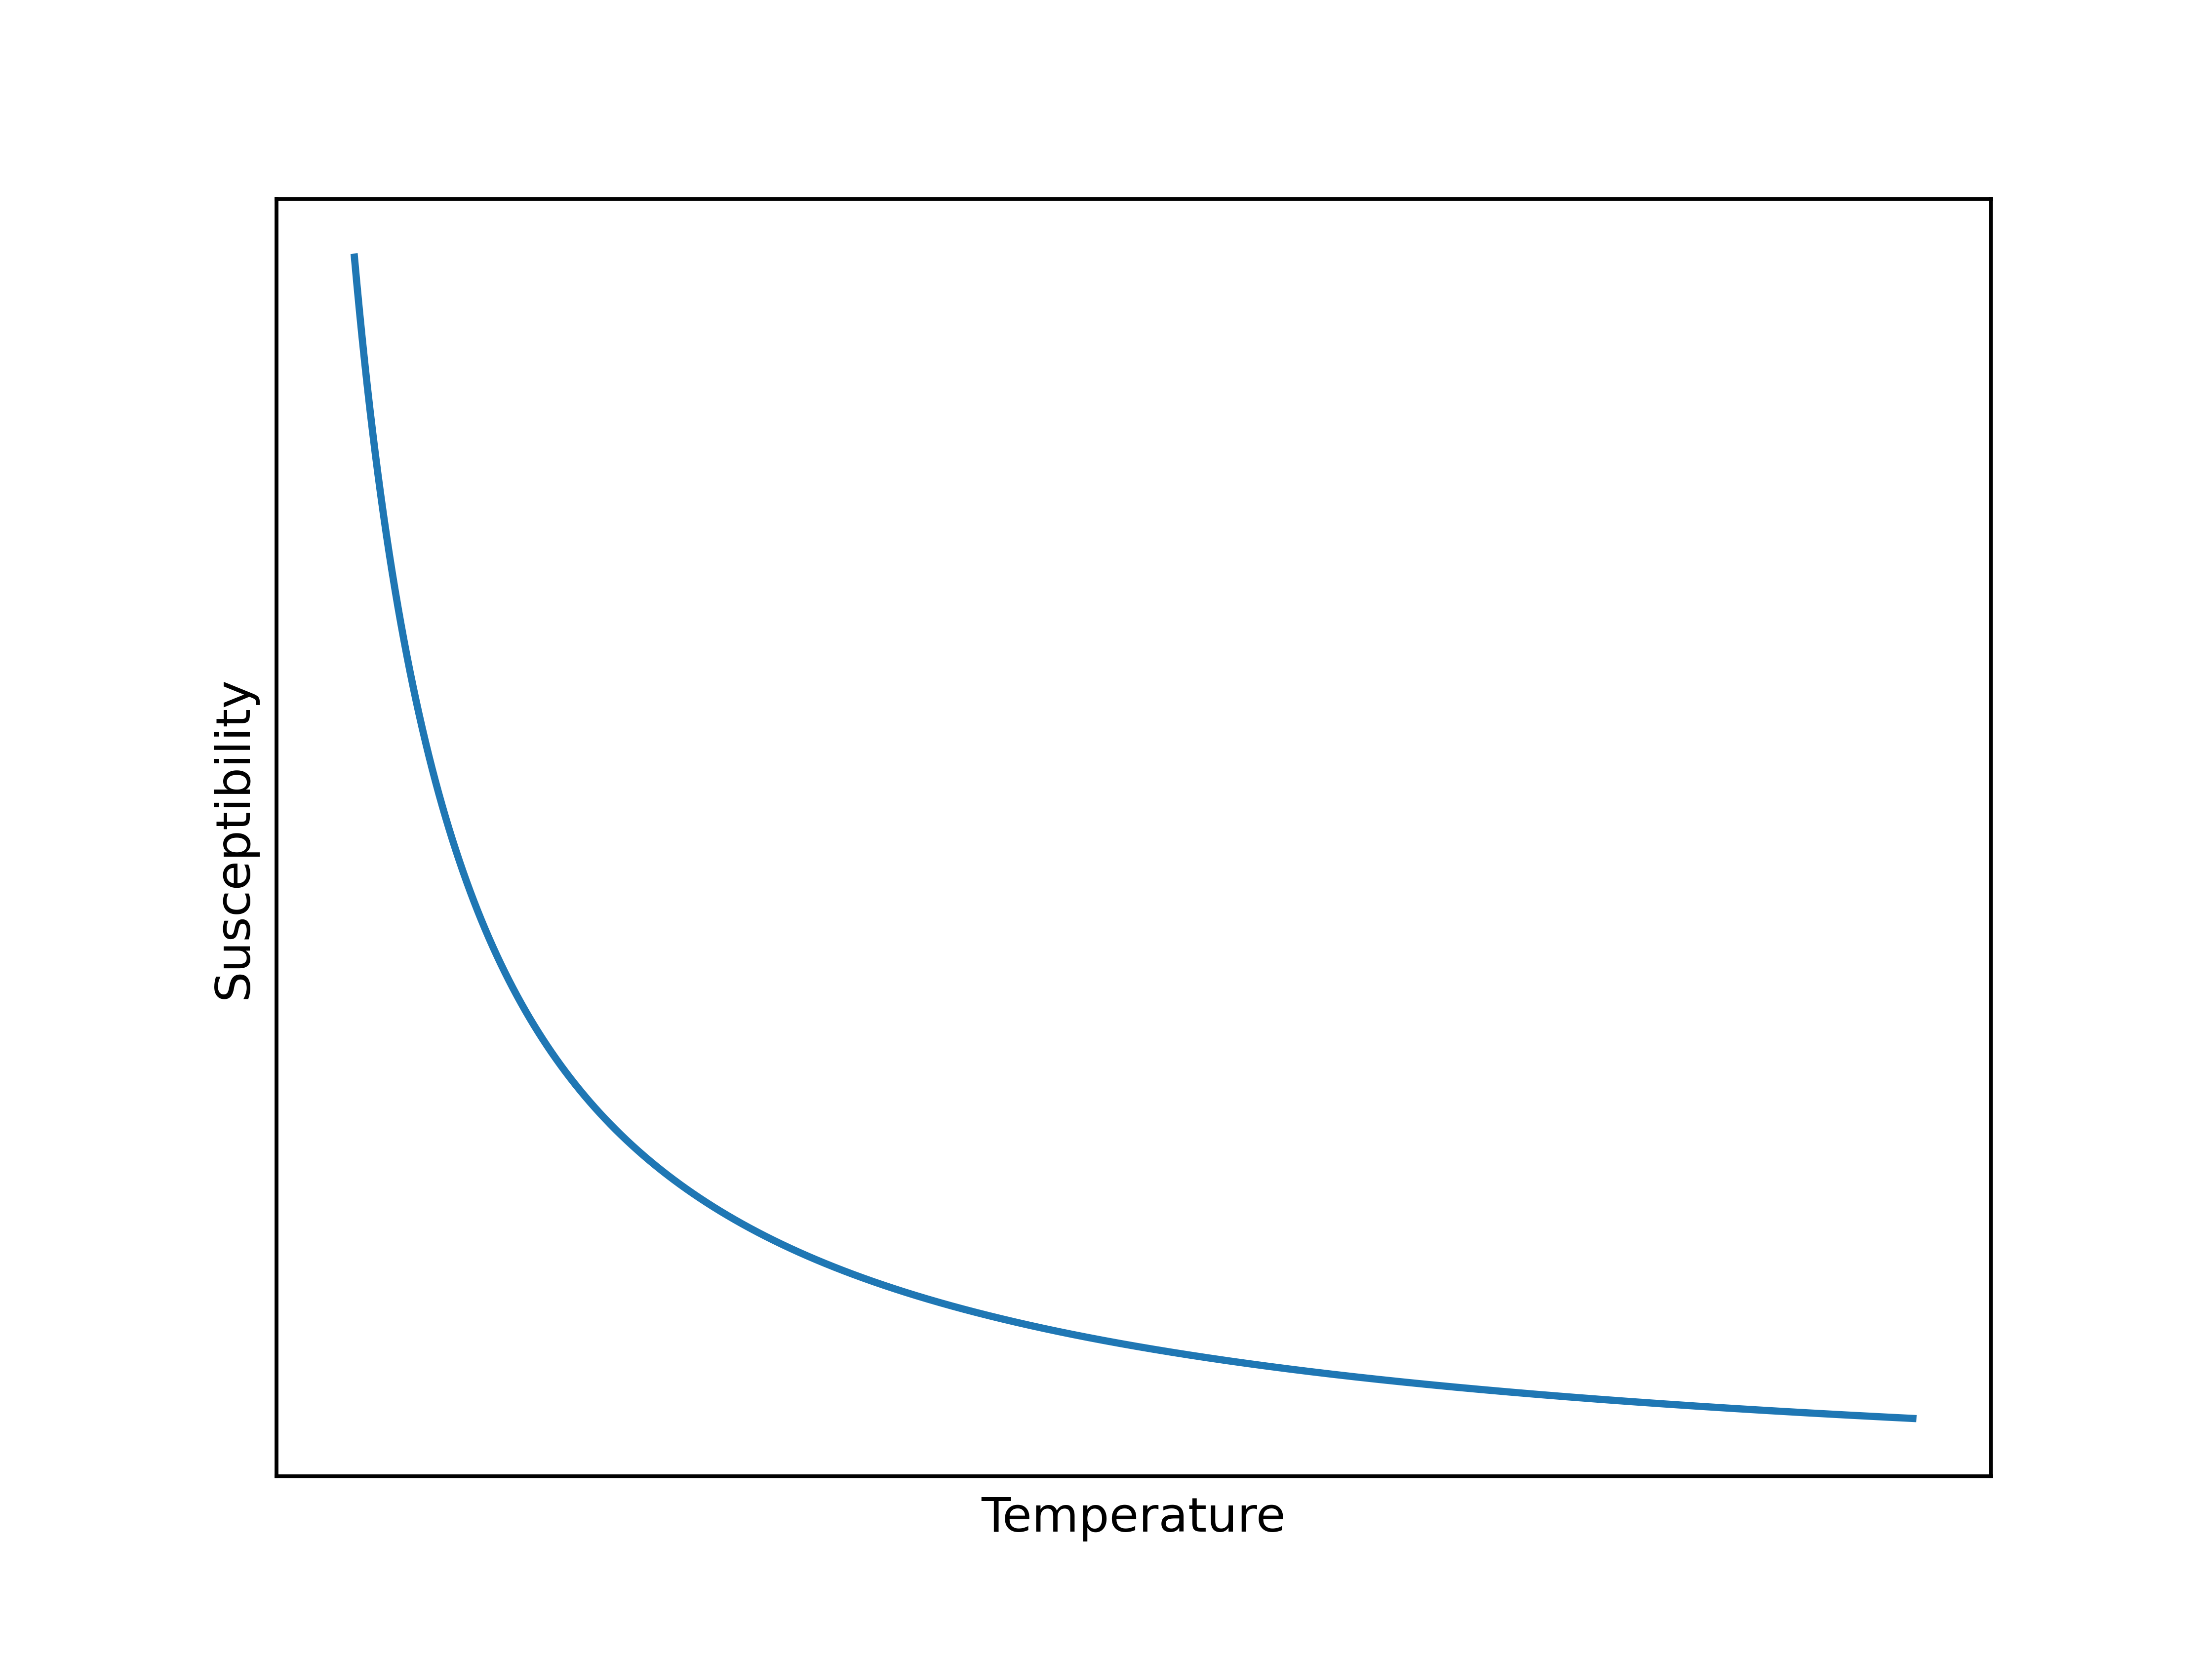
\includegraphics[width=0.9\linewidth]{inverse.png}
  \caption{Curie's law which shows inverse temperature relationship}
\end{figure}
\\
\item Pauli paramagnetism: For some alkali metals and noble metals, conduction electrons are weakly interacting and delocalized in space forming a Fermi gas. For these materials one contribution to the magnetic response comes from the interaction between the electron spins and the magnetic field known as Pauli paramagnetism. \cite{wikipara}

\end{itemize}

The Bohr–Van Leeuwen theorem proves that there cannot be any diamagnetism or paramagnetism in a purely classical system.\cite{wikipara}

\subsubsection{Diamagnetic materials}

Diamagnetic materials have opposite magnetization to applied fields. Thus they are repelled by magnets. Diamagnetic properties always exist in material but when compared with strong magnetic properties of the same material it is negligible. They have negative magnetic susceptibility and are very negligible. Superconductors also show diamagnetism, which have very high but negative susceptibility, $\chi \approx -1$ (in SI units). This can be understood by the Meissner effect. Certain theories are made for understanding diamagnetism. They are Lengevin’s theory and Landau’s theory which we will not go deeper.\cite{wikidia}

\subsubsection{Ferromagnetic materials}
Ferromagnetic materials have by far the most visible magnetic effect compared to diamagnetic and paramagnetic materials. These materials are highly attracted to applied magnetic fields, thus having high magnetic susceptibility. Compared to paramagnets and diamagnets, ferromagnets' magnetic susceptibility is easily measured at some degree of accuracy because of its high value. In our project we are focusing on ferromagnets and their phase transitions because of noise factors. Some examples of ferromagnets are iron, nickel, cobalt, LSMO etc.. There’s similar classification for ferromagnetic and antiferromagnetic materials, the difference being how spins are aligning throughout. \cite{wikiferro}

\subsection{Magnetic phase transition}

By data of magnetic susceptibility we can study magnetic phase transition. With temperature magnetic properties such as paramagnetism, diamagnetism etc. changes. This is an almost sudden change with temperature. With studying susceptibility data we can pinpoint from which temperature change has occurred. This temperature is called Curie Temperature.

\begin{figure*}
\centering\includegraphics[width=\textwidth, page=5, trim={1cm 22cm 1cm 1.2cm}, clip ]{phasefig.pdf}
\caption{This is phase transition for different materials with magnetic classification. Relations are related with temperature, you can measure curie temperature for different materials which will directly relate to phase transition.\cite{Mugiraneza2022}}
\label{fig:phasefig}
\end{figure*}

Certain material types have unique phase transition properties. For example, Superconductors are almost perfect diamagnet at their superconducting state and almost none magnetic(for most of the compound superconductors) after critical temperature $T_c$. You can see certain phase relationships in figure \ref{fig:phasefig}\cite{Mugiraneza2022}. 

\subsection{AC susceptibility vs DC susceptibility}
We can measure susceptibility values in two different ways. First is after applying a DC magnetic field and second is after applying AC magnetic field. Difference is first you will measure $\chi_{DC} = \frac{M}{H}$ where second $\chi_{AC} = \frac{dM}{dH}$.
AC magnetic fields will generate loss terms because of changing magnetic fields of the sample. 

$\chi= \chi^\prime +\chi^{\prime\prime}$

AC susceptibility will depend on frequency of applied field. Also, if we can measure phase change of applied magnetic field and sample magnetic field, we will see frequency dependent relationships. For example look at figure \ref{fig:phaserel}.

\begin{figure}
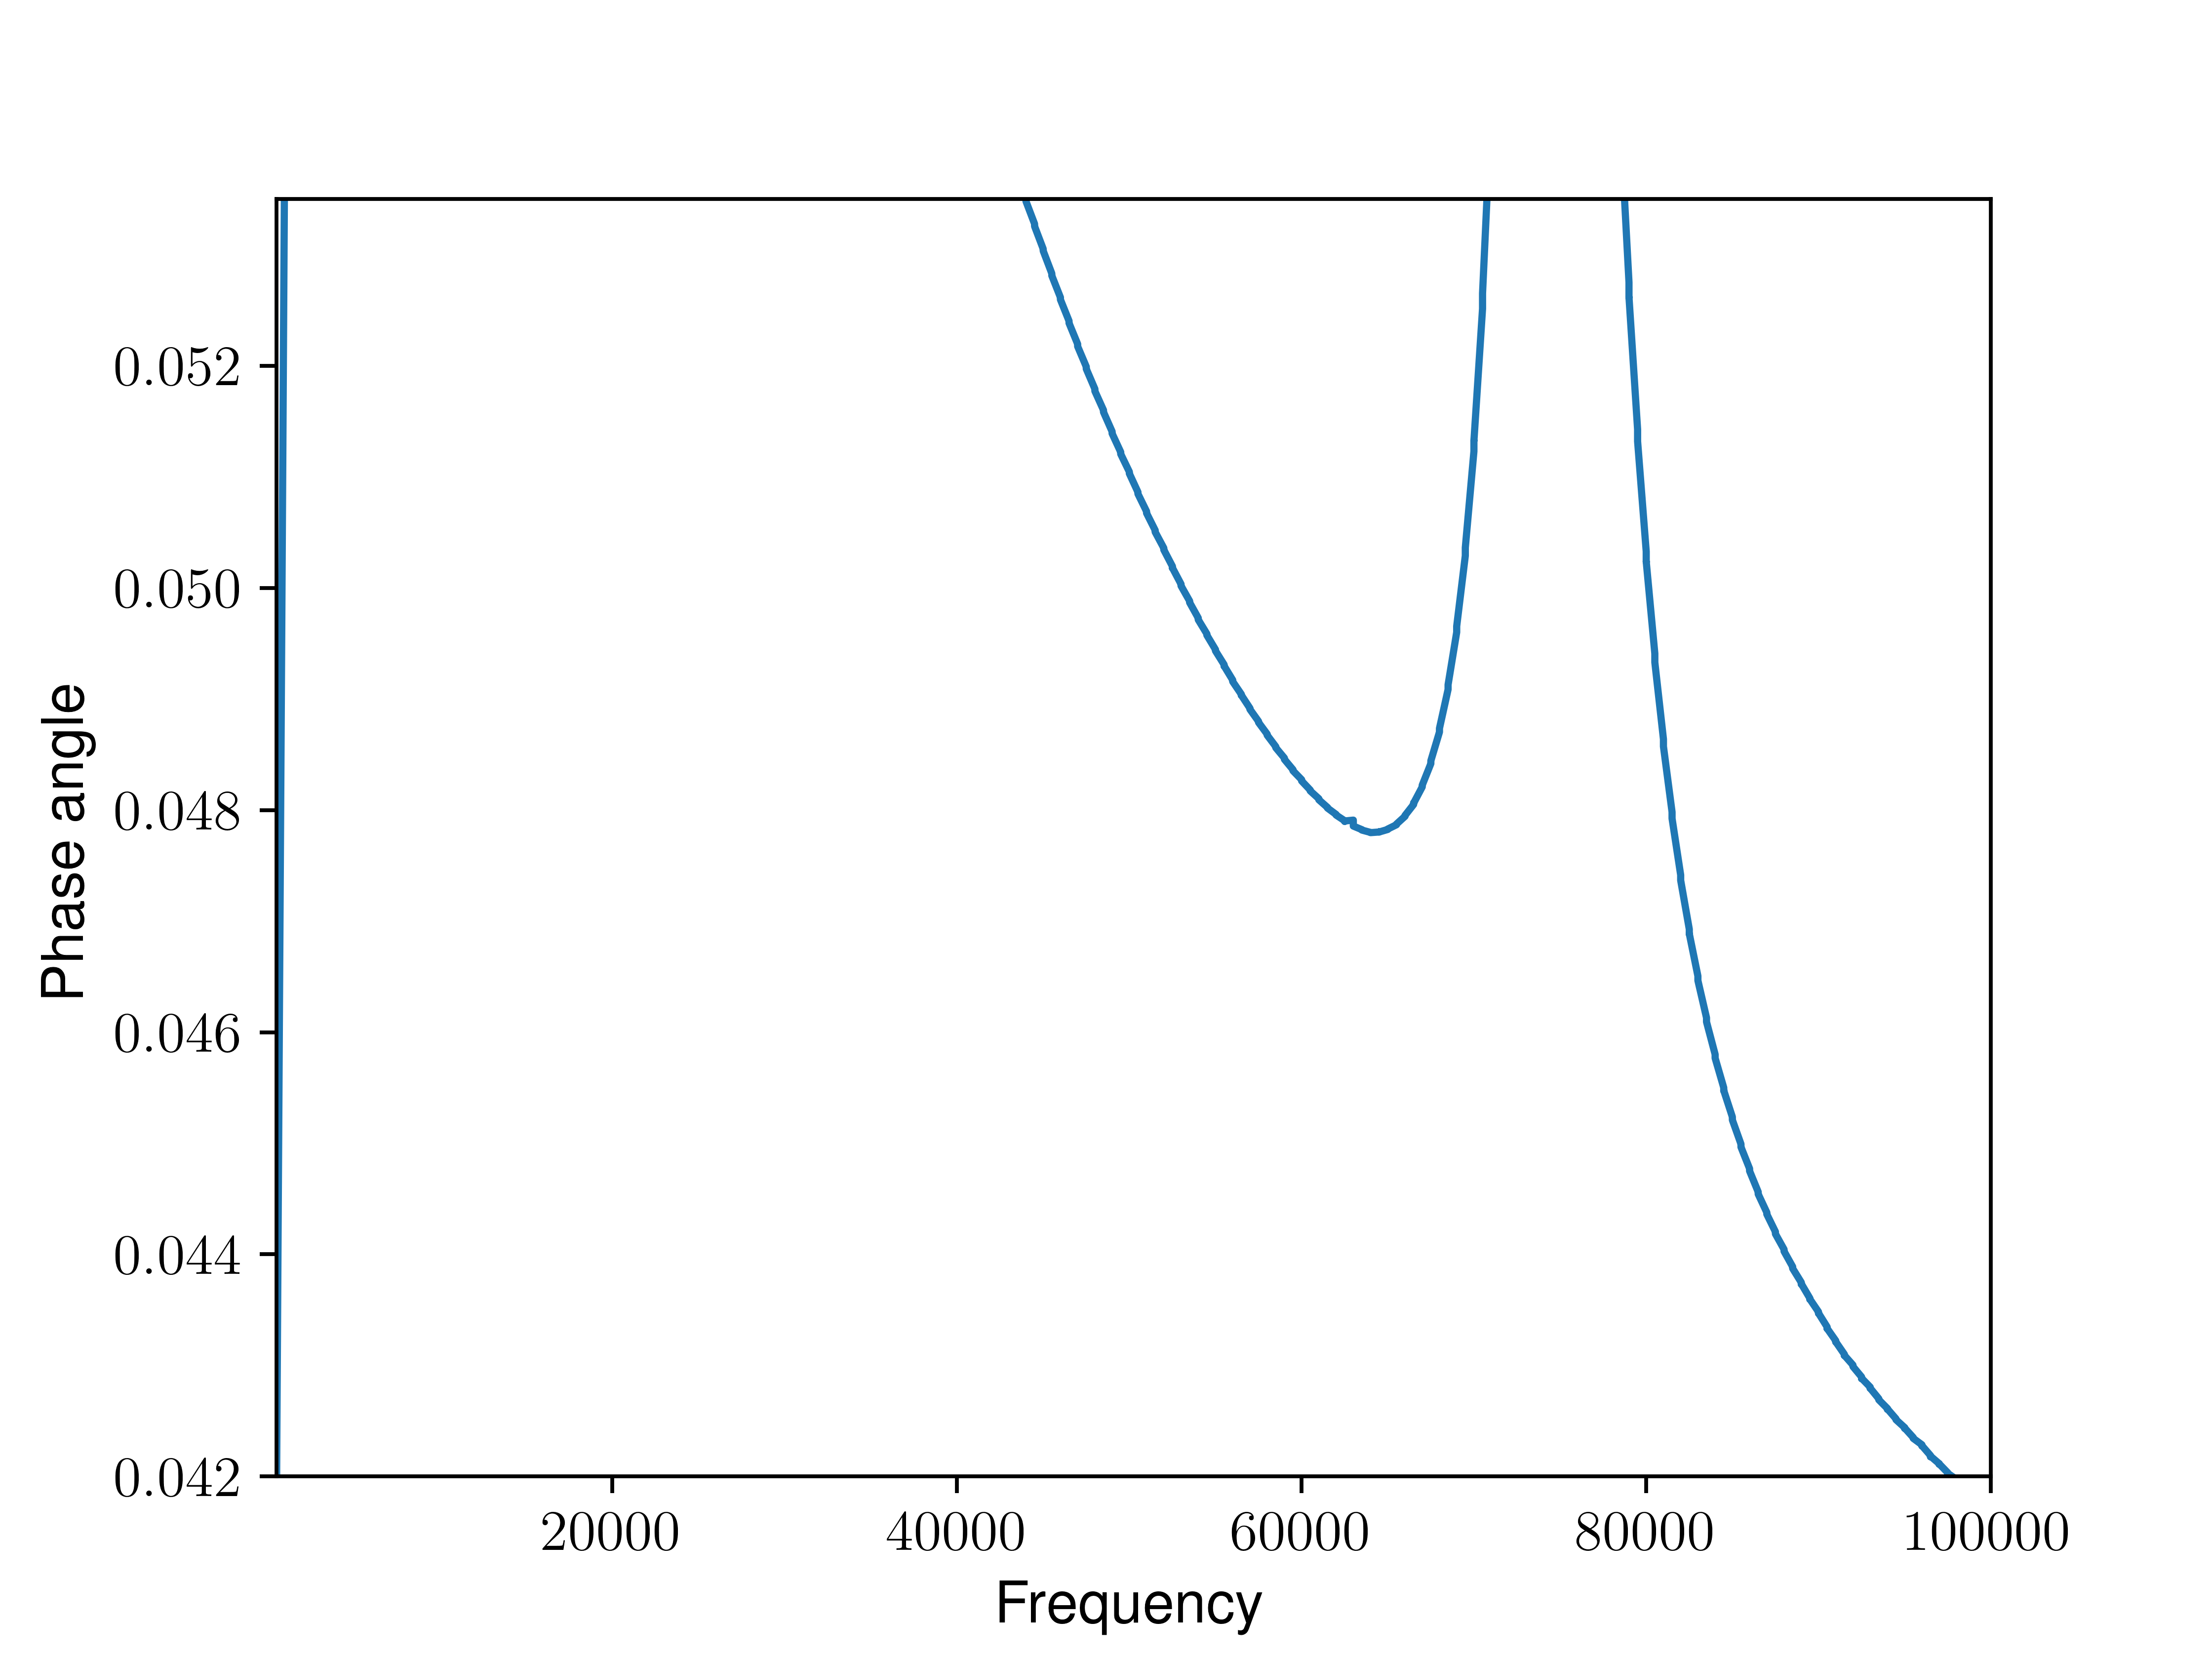
\includegraphics[width=\linewidth]{phaserel.png}
\caption{Phase relation with frequency for Iron rod}
\label{fig:phaserel}
\end{figure}

After knowing the importance of why it is important to measure magnetic susceptibility we will devise instrumentation techniques to measure magnetic susceptibility at given temperature and frequency. This will give insight into magnetic phase transition and sample's magnetic properties.

%% \subsection{Magnetism}

%% We should know little about some concepts of magnetism. Magnetism in loops is profoundly due to relative motions of charge particles. This is related to concepts of relativity (especially Einstein’s special relativity). As we know moving charge creates a magnetic field which curls around movement direction. These magnetic fields get accumulated with a number of loops which relate to our instrumentations. Also, changing velocity (relates directly to changing current) creates a changing magnetic field.

%% There’s another type of magnetism which differs in some minor differences. This is related to the material’s magnetic moments. As we know atoms have magnetic moments related with two momentums, orbital angular momentum and spin angular momentum. This degree of freedom of electrons (as by product relates to atoms) creates magnetic properties of materials. 

%% \subsection{Spins}

%% First evident by an experiment in 1922 by Otto Stern and Walther Gerlach. \cite{stern} As Experiment showed that magnetic moments must be quantized. As it turns out this is an extra degree of freedom giving physics a new direction.
%% Magnetic moment by this spins is as following,

%% \begin{equation*}
%% \mu = g \frac{e \hbar}{2m_e}\frac{S}{\hbar}
%% \end{equation*}



%% A magnetic susceptibility of a material can be defined as the amount of a material that gets magnetised, when it is placed in an external magnetic field. In other words, an amount of magnetization of a material occurs when it is placed in an external magnetic field .

%% An expression for magnetic susceptibility is given by ,

%% \begin{equation*}
%%   \chi = \frac{M}{H}
%% \end{equation*}


%% Where , M= Magnetic susceptibility, H= Applied/External magnetic field 

%% There are two other measures of susceptibility:
%% 1. Magnetic molar susceptibility ($\chi_m$)
%% 2. Mass magnetic susceptibility ($\chi_p$)
                   
%% \begin{equation*}
%% \chi_m = M \chi_р
%% \end{equation*}

%% Where,  $\chi_р = \frac{\chi_V}{p}$ , р= density ($\frac{kg}{m^3}$)

%% Magnetic susceptibility is a factor that indicates the magnetic behaviour of a material. It gives an idea about a material that it can attract or repel. 

%% subsection{Classification of magnetic material based on their magnetic properties}
%% Materials have very distinct and condition dependent magnetic properties. This material is broadly classified in certain classes with its magnetic susceptibility and its relation with temperature. With this we represent certain classes dependent on their magnetic properties.

%% \subsubsection{Diamagnetic material}

%% A magnetic material which aligns its domains or field lines against the applied magnetic field are known as diamagnetic materials. These materials are strongly repelled by the magnets. As these materials get magnetised on the opposite side of the applied field, they have a small amount of magnetization. They have magnetic susceptibility Χ < 0, negative value of magnetic susceptibility.

%% Example :- water, tin , mercury ,etc.

%% \subsubsection{Paramagnetic material} :

%% A magnetic material which aligns its domains or field lines with the applied field are known as paramagnetic materials. These materials are weakly attracted by the magnets and also they are temperature dependent. They have magnetic susceptibility Χ > 0, positive value of magnetic susceptibility (which is very small value).

%% Example :- aluminium, alkaline earth metals, etc.


%% \subsubsection{Ferromagnetic materials}:

%% Magnetic materials that are highly magnetised in an external magnetic field are known as ferromagnetic materials. These materials are highly attracted by the magnets. They have magnetic susceptibility Χ > 1, always higher value of magnetic susceptibility.

%% Example :- iron, cobalt, nickel , etc .

 
%% There are further classification of materials based on their magnetic properties can be done as :

%% a) Anti-ferromagnetic materials 

%% b) Ferrimagnetic materials 

%% These two types are not discussed in detail because they are not in context to our project work .

%% \subsection{What do you mean by an ac magnetic susceptibility ?}

%% AC magnetic measurements are taken by applying AC field to the samples and resulting AC magnetic moment is measured i.e.,
%% induced by changing magnetic flux by applied AC field .

%% This results in the different values of magnetic susceptibility for different values of magnetic flux arising from the different values of the AC field.

%% In order to understand AC magnetic susceptibility , first we have consider measurements at low frequencies , where the 
%% measurements is almost equals to the DC susceptibility.In this case the absolute value of magnetization is calculated i.e.,

%% \begin{equation*}
%% \chi = \frac{M}{H}
%% \end{equation*}

%% In case of AC susceptibility, the continuously varying value of magnetization , hence varying value of susceptibility i.e.,

%% \begin{equation*}
%% \chi_{AC} = \frac{dM}{dH}
%% \end{equation*}

%% AC susceptibility is often referred to as dynamic susceptibility.AC measurements are very sensitive to the small changes in the values of magnetization .
